%++++++++++++++++++++++++++++++++++++++++++++++++
\section{Appariement}
%------------------------------------------------
\begin{frame}{Le problème de l'appariement}
  \note{
     Une fois les coins détectés dans deux images différentes, l’objectif est de retrouver les correspondances entre eux.
C’est ce qu’on appelle l’appariement.
  }
  \begin{minipage}{0.48\linewidth}
    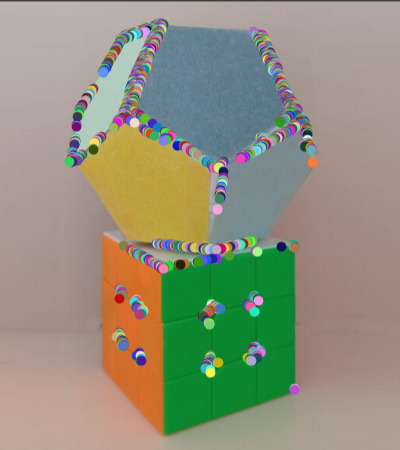
\includegraphics[width=\linewidth]{capture/test_detection_1_moravec_2_500.jpeg}  
  \end{minipage}
  \hfill
    \begin{minipage}{0.48\linewidth}
    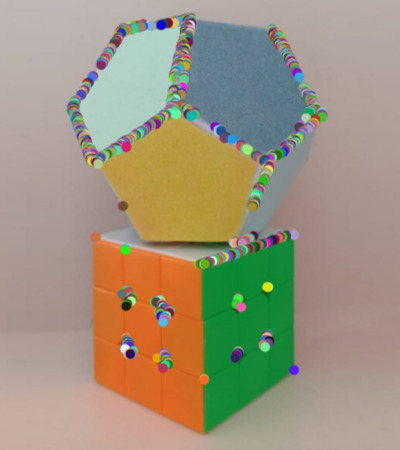
\includegraphics[width=\linewidth]{capture/test_detection_img2_1_moravec_2_500.jpeg}
  \end{minipage}
\end{frame}

\begin{frame}{Le problème de l'appariement}
    \note{
  Par exemple si l'on a deux images avec les points detectés comme ceci
  On remarque par ailleurs qu'il n'y a ni injectivité, ni surjectivité. Notre but est certe de garder un maximum de points mais le plus important est d'éviter tout erreur d'appariement qui peut completement fausser la reconstrution dans le calcul de l'enveloppe convexe.
  }

\centering
\begin{tikzpicture}[scale=1]

% Boîtes des images
\draw[thick] (0,0) rectangle (3,4) node[midway] {Image 1};
\draw[thick] (6,0) rectangle (9,4) node[midway] {Image 2};

% Points en gris par défaut
\fill[gray] (0.8,3.5) circle (2pt); % rouge
\fill[gray] (1.2,2.7) circle (2pt); % vert
\fill[gray] (1.5,1.8) circle (2pt); % bleu foncé
\fill[gray] (1.0,1.0) circle (2pt); % bleu clair
\fill[gray] (1.4,1.4) circle (2pt);

\fill[gray] (7.5,3.3) circle (2pt);
\fill[gray] (7.8,2.5) circle (2pt);
\fill[gray] (7.4,3.0) circle (2pt);
\fill[gray] (8.4,1.0) circle (2pt);
\fill[gray] (8.0,1.6) circle (2pt);
\fill[gray] (8.6,3.6) circle (2pt);
\fill[gray] (8.3,3.1) circle (2pt);
\fill[gray] (7.3,0.9) circle (2pt);
\fill[gray] (6.3,0.6) circle (2pt);

% Paire 1 - rouge
\only<2->{%
  \fill[red]   (0.8,3.5) circle (2pt);
  \fill[red]   (7.5,3.3) circle (2pt);
  \draw[->,red,thick]   (0.8,3.5) -- (7.5,3.3);
}

% Paire 2 - vert foncé
\only<3->{%
  \fill[green!50!black] (1.2,2.7) circle (2pt);
  \fill[green!50!black] (7.8,2.5) circle (2pt);
  \draw[->,green!50!black,thick] (1.2,2.7) -- (7.8,2.5);
}

% Paire 3 - bleu foncé
\only<4->{%
  \fill[blue!70!black]  (1.5,1.8) circle (2pt);
  \fill[blue!70!black]  (8.0,1.6) circle (2pt);
  \draw[->,blue!70!black,thick]  (1.5,1.8) -- (8.0,1.6);
}

% Paire 4 - bleu clair
\only<5->{%
  \fill[cyan]  (1.0,1.0) circle (2pt);
  \fill[cyan]  (7.3,0.9) circle (2pt);
  \draw[->,cyan,thick]  (1.0,1.0) -- (7.3,0.9);
}

\end{tikzpicture}

\end{frame}
%===========================
\subsection{Pré-traitement}
%===========================

\begin{frame}{Pré-traitement}
  \note{une première étape consiste à effectuer un traitement des points détecter par Moravec
  Ce traitement est réalisé à l'aide d'un premier algorithme "trouve coin" basé sur la rechercche d'extrema locaux implémenté par mon camarade
  Un second algorithme de type Ransac permet d'identifier les points alignés et d'éliminer ceux sur une même droite
  }
    \begin{center}
    \begin{minipage}{0.32\textwidth}
        \onslide<1->{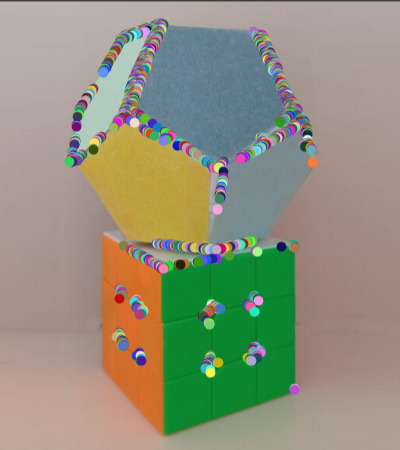
\includegraphics[width=\linewidth]{capture/test_detection_1_moravec_2_500.jpeg}\\
        \centering\scriptsize Sélection}
    \end{minipage}
    \hfill
    \begin{minipage}{0.32\textwidth}
        \onslide<2->{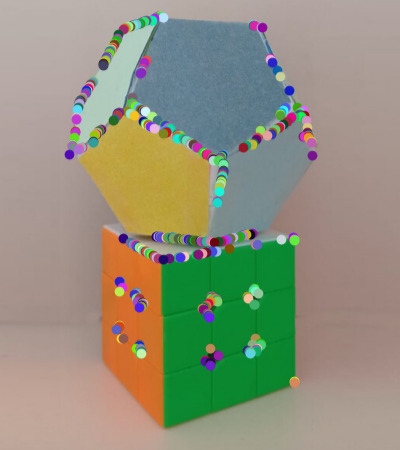
\includegraphics[width=\linewidth]{capture/test_detection_2_trouve_coin_10_500.jpeg}\\
        \centering\scriptsize Trouve coin}
    \end{minipage}
    \hfill
    \begin{minipage}{0.32\textwidth}
        \onslide<3->{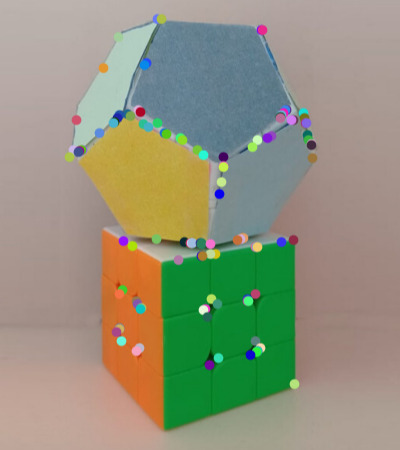
\includegraphics[width=\linewidth]{capture/test_detection_3_ransac_1000_6_5.jpeg}\\
        \centering\scriptsize Ransac
        \hyperlink{ransac-appendix}{
    \beamerbutton{Explication Ransac}
  }}

    \end{minipage}
    \end{center}

\end{frame}

\begin{frame}{Appariement}
  \note{
    On ne traite que l image 1 pour ne pas enlever de potentiels match
    On peut désormais effectuer l eppariement
  }
  \begin{minipage}{0.48\linewidth}
    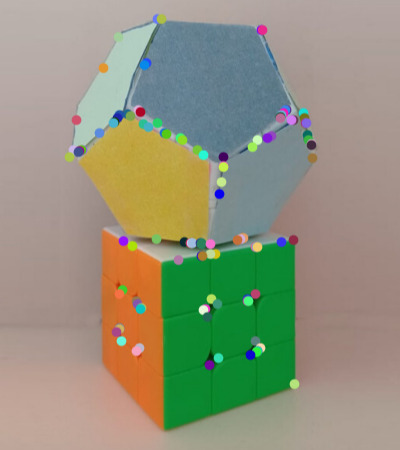
\includegraphics[width=\linewidth]{capture/test_detection_3_ransac_1000_6_5.jpeg}  
  \end{minipage}
  \hfill
    \begin{minipage}{0.48\linewidth}
    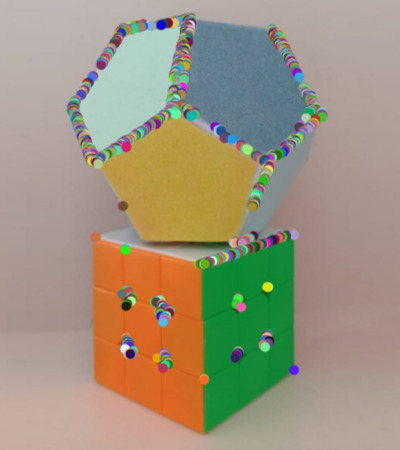
\includegraphics[width=\linewidth]{capture/test_detection_img2_1_moravec_2_500.jpeg}
  \end{minipage}
\end{frame}
%===========================
\subsection{Filtrage epipolaire}
%===========================

\begin{frame}{Geometrie epipolaire}
\note{J’introduis ici la géométrie épipolaire : lorsque deux caméras observent une même scène, les points correspondants sont contraints de vérifier une relation géométrique.
Les deux caméras ont pour centres optiques respectifs C1 et C2 et pour plans-images P1 et P2. Pour des raisons de lisibilité, les plans-
images sont placés dans ce schéma devant les centres optiques. Un point M de la scène
se projette sur le plan-image de la caméra 1 (resp. 2) en m1 (resp. m2). Le point e1
(resp. e2) est l’image de C2 (resp. C1) sur P1 (resp. P2). Les points e1 et e2 sont appelés
épipoles. La droite l1 (resp. l2) joignant les points e1 et m1 (resp. e2 et m2) est appelée
droite épipolaire associée à m2 (resp. m1).
C’est cette contrainte qui nous permettra de filtrer les correspondances incorrectes.
Elle est encodé sous forme d'une matrice qu'on détermine à l'étape de calibration expliquéé ultérieurement}
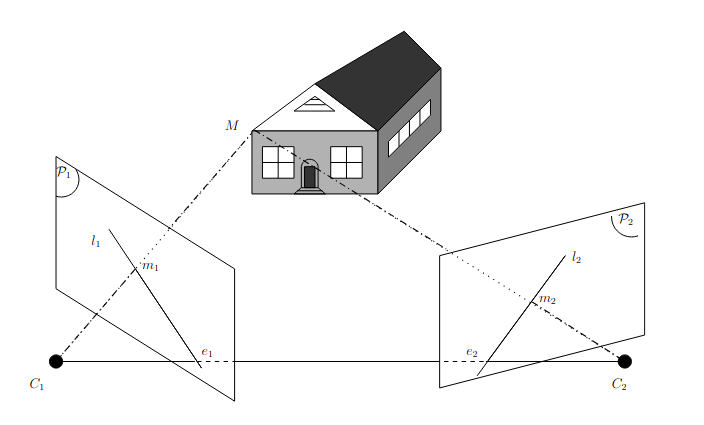
\includegraphics[width=\linewidth]{capture/geom-epipolaire.png}\\[0.5em]
\tiny
Source image: Quelques problèmes géométriques
en vision par ordinateur - Frédéric SUR
\end{frame}

\begin{frame}{Filtrage epipolaire}
  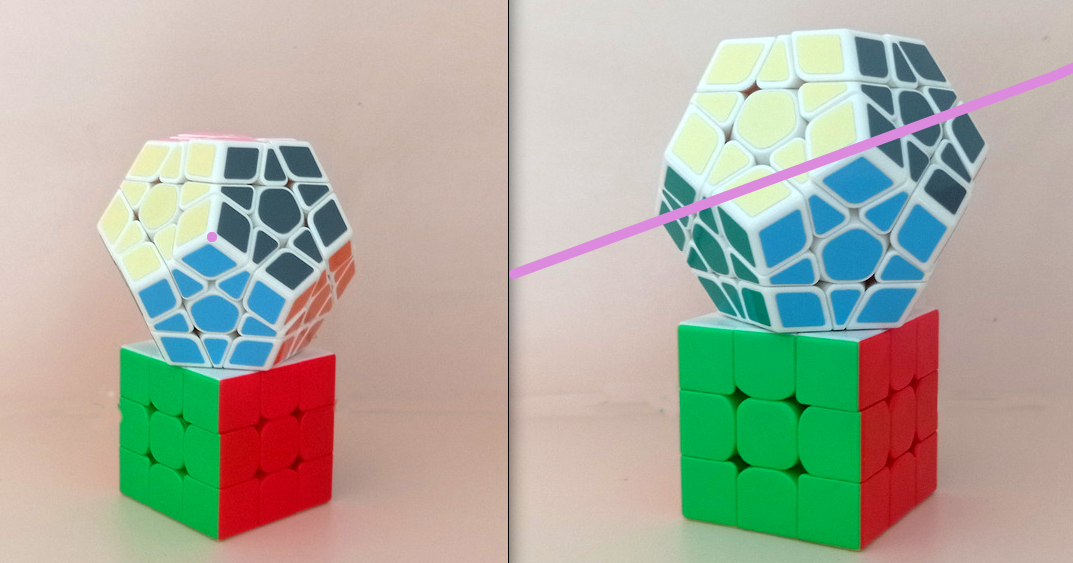
\includegraphics[width=\linewidth]{capture/ligne.png}\\[0.5em]
  \captionof*{figure}{Droite epipolaire}
\end{frame}


%===========================
\subsection{Descripteur}
%===========================

% \begin{frame}{Descripteur BRIEF : Principe}
% \begin{minipage}{0.45\linewidth}
% \begin{tikzpicture}[x=1pt,y=1pt,yscale=-1,xscale=1, scale= 0.6]
%     % Grille gauche
%     \draw[step=20,gray!30,thin] (100,20) grid (320,240);
%     \fill[black] (200,120) rectangle ++(20,20);

%     % Étape 1 : Choix de paires de pixels
%     \only<2->{\fill[blue]     (100,60)  rectangle ++(20,20);}
%     \only<3->{\fill[green]    (180,220) rectangle ++(20,20);}
%     \only<4->{\fill[orange]   (200,100) rectangle ++(20,20);}
%     \only<4->{\fill[violet]   (140,100) rectangle ++(20,20);}
%     \only<5->{\fill[pink]     (240,60)  rectangle ++(20,20);}
%     \only<5->{\fill[teal]     (260,140) rectangle ++(20,20);}
%     \only<6->{\fill[yellow]   (140,180) rectangle ++(20,20);}
%     \only<6->{\fill[magenta]  (220,180) rectangle ++(20,20);}
%     \only<7->{\fill[cyan]     (240,200) rectangle ++(20,20);}
%     \only<7->{\fill[red]      (280,20)  rectangle ++(20,20);}
% \end{tikzpicture}
% \end{minipage}
% \hfill
% \begin{minipage}{0.45\linewidth}
% \small
% \textbf{Comparaisons binaires :}
% \begin{tabbing}
% \only<3->{\textcolor{blue}{Bleu} < \textcolor{green}{Vert} \quad \= ~~~~$\Rightarrow$ \texttt{1} \kill} % pour alignement
% \only<3->{\textcolor{blue}{Bleu} < \textcolor{green}{Vert} \> ~~~~$\Rightarrow$ \texttt{1}}\\
% \only<4->{\textcolor{orange}{Orange} > \textcolor{violet}{Violet} \> ~~~~$\Rightarrow$ \texttt{0}}\\
% \only<5->{\textcolor{pink}{Rose} < \textcolor{teal}{Turquoise} \> ~~~~$\Rightarrow$ \texttt{1}}\\
% \only<6->{\textcolor{yellow}{Jaune} > \textcolor{magenta}{Magenta} \> ~~~~$\Rightarrow$ \texttt{0}}\\
% \only<7->{\textcolor{cyan}{Cyan} < \textcolor{red}{Rouge} \> ~~~~$\Rightarrow$ \texttt{1}}
% \end{tabbing}

% \vspace{1em}
% \only<8->{%
% \textbf{Descripteur final :}\\
% \texttt{1 0 1 0 1}
% }
% \end{minipage}
% \vspace{1em}

% \begin{itemize}
%   \item<1-> On considère une fenêtre autour d’un point clé.
%   \item<2-> On choisit aléatoirement un pixel (ex: \textcolor{blue}{bleu}).
%   \item<3-> On la compare à un autre (ex: \textcolor{green}{vert}) : \\
%            $\text{BRIEF}_1 = 1$ si intensité(bleu) < intensité(vert)
%   \item<4-> On répète avec d'autres paires (ex: \textcolor{orange}{orange} vs \textcolor{violet}{violet})...
% \end{itemize}
% \end{frame}

\begin{frame}{Descripteur BRIEF : Principe}
\begin{minipage}{0.45\linewidth}
\begin{tikzpicture}[x=1pt,y=1pt,yscale=-1,xscale=1, scale= 0.6]
    % Grille de fond
    \draw[step=20,gray!30,thin] (100,20) grid (320,240);

    % Centre de la fenêtre
    \fill[blue] (200,120) rectangle ++(20,20);

    % Comparaisons (coordonnées relatives)
    \only<2->{\fill[gray!50] (100,60)  rectangle ++(20,20);}
    \only<3->{\fill[gray!80] (180,220) rectangle ++(20,20);}
    \only<4->{\fill[gray!60] (200,100) rectangle ++(20,20);}
    \only<4->{\fill[gray!30] (140,100) rectangle ++(20,20);}
    \only<5->{\fill[gray!40] (240,60)  rectangle ++(20,20);}
    \only<5->{\fill[gray!70] (260,140) rectangle ++(20,20);}
    \only<6->{\fill[gray!85] (140,180) rectangle ++(20,20);}
    \only<6->{\fill[gray!20] (220,180) rectangle ++(20,20);}
    \only<7->{\fill[gray!35] (240,200) rectangle ++(20,20);}
    \only<7->{\fill[gray!65] (280,20)  rectangle ++(20,20); }
\end{tikzpicture}
\end{minipage}
\hfill
\begin{minipage}{0.45\linewidth}
\small
\textbf{Comparaisons binaires :}
\begin{tabbing}
\only<3->{I(-5,-3) < I(-1,5) \quad \= ~~~~$\Rightarrow$ \texttt{1} \kill}
\only<3->{I(-5,-3) < I(-1,5) \> ~~~~$\Rightarrow$ \texttt{1}}\\
\only<4->{I(0,-1) > I(-3,-1) \> ~~~~$\Rightarrow$ \texttt{0}}\\
\only<5->{I(2,-3) < I(3,1) \> ~~~~$\Rightarrow$ \texttt{1}}\\
\only<6->{I(-3,3) > I(1,3) \> ~~~~$\Rightarrow$ \texttt{0}}\\
\only<7->{I(2,4) < I(4,-5) \> ~~~~$\Rightarrow$ \texttt{1}}
\end{tabbing}

\vspace{1em}
\only<8->{%
\textbf{Descripteur final :}\\
\texttt{1 0 1 0 1}
}
\end{minipage}
\vspace{1em}

\begin{itemize}
  \item<1-> On considère une fenêtre autour d’un point clé, ici le centre $(0,0)$.
  \item<2-> On choisit aléatoirement un pixel (ex: \texttt{(-5,-3)}).
  \item<3-> On le compare à un autre (ex: \texttt{(-1,5)}) :\\
           $\text{BRIEF}_1 = 1$ si intensité(1er) < intensité(2e)
  \item<4-> On répète avec d'autres paires...
\end{itemize}
\end{frame}


\begin{frame}{Amélioration progressive du descripteur BRIEF}
\small

\textbf{1. BRIEF (intensité)} \\
\hspace{1em}• Comparaison d’intensité de pixels en niveaux de gris \\
\hspace{1em}• \textit{Simple et rapide, mais perte d'information sur la couleur} \\

\pause
\vspace{0.5em}
\textbf{2. BRIEF RGB} \\
\hspace{1em}• Comparaison faite indépendamment sur les 3 canaux : R, G, B \\
\vspace{0.5em}
\hspace{1em}
\begin{minipage}{\linewidth}
\centering
\setlength{\fboxsep}{0pt}
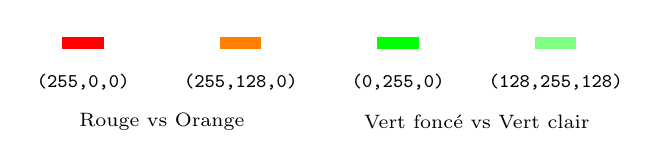
\begin{tikzpicture}
% Rouge vs Orange
\node at (0, 0) {\colorbox[RGB]{255,0,0}{\phantom{aaa}}};
\node at (2, 0) {\colorbox[RGB]{255,128,0}{\phantom{aaa}}};
\node at (0, -0.5) {\scriptsize \texttt{(255,0,0)}};
\node at (2, -0.5) {\scriptsize \texttt{(255,128,0)}};
\node at (1, -1) {\scriptsize Rouge vs Orange};

% Vert foncé vs Vert clair
\node at (4, 0) {\colorbox[RGB]{0,255,0}{\phantom{aaa}}};
\node at (6, 0) {\colorbox[RGB]{128,255,128}{\phantom{aaa}}};
\node at (4, -0.5) {\scriptsize \texttt{(0,255,0)}};
\node at (6, -0.5) {\scriptsize \texttt{(128,255,128)}};
\node at (5, -1) {\scriptsize Vert foncé vs Vert clair};
\end{tikzpicture}
\end{minipage}

\vspace{0.8em}
\hspace{1em}• \textit{→ RGB ne reflète pas toujours la perception humaine}

\pause
\vspace{0.5em}
\textbf{3. BRIEF Lab} \\
\hspace{1em}• Comparaison dans l’espace Lab : \\
\hspace{2em}– $L$ : luminosité (luminance) \\
\hspace{2em}– $a$, $b$ : composantes de couleur perceptuelles \\

\end{frame}
\begin{frame}{Comparaison de descripteurs BRIEF : distance de Hamming}
\centering
\small
\note{Plus la distance est faible, plus les points sont similaires.}

\textbf{Descripteur 1 (image gauche)}\\[0.2em]
\texttt{1 \quad 0 \quad 1 \quad 0 \quad 1}
\pause

\vspace{0.8em}
\textbf{Descripteur 2 (image droite)}\\[0.2em]
\texttt{1 \quad 1 \quad 0 \quad 0 \quad 1}
\pause

\vspace{1em}
\textbf{Comparaison bit à bit :}\\[0.5em]
\begin{tabular}{c}
\begin{tabular}{c c c c c}
\textbf{Bit 1} & \textbf{Bit 2} & \textbf{Bit 3} & \textbf{Bit 4} & \textbf{Bit 5} \\
1 & 0 & 1 & 0 & 1 \\
1 & 1 & 0 & 0 & 1 \\
\hline
\textcolor{green}{0} & \textcolor{red}{1} & \textcolor{red}{1} & \textcolor{green}{0} & \textcolor{green}{0}
\end{tabular}
\end{tabular}
\pause

\vspace{1em}
\textbf{Distance de Hamming = nombre de bits différents = } \texttt{2}

\end{frame}


%===========================
\subsection{Algorithme}
%===========================

\begin{frame}[fragile]{Pseudo-code : Appariement de points}
  \scriptsize
\begin{algorithm}[H]
\DontPrintSemicolon
\Input{Points $P_1$ sur image 1, Points $P_2$ sur image 2, Matrice fondamentale $F$}
\Output{Liste de correspondances fiables}
\BlankLine
\textbf{Pré-tri des points sur image 1} \;
\ForEach{$p \in P_1$}{
    \Si{$p$ n'est pas un coin}{
        retirer $p$ \tcp*{suppression non maximale locale}
    }
}

\BlankLine
\textbf{Filtrage épipolaire} \;
\ForEach{$p_1 \in P_1$}{
    $l \gets F \cdot p_1$ \tcp*{droite épipolaire dans image 2}
    $C(p_1) \gets \{p_2 \in P_2 \mid \text{distance}(p_2, l) < \varepsilon\}$ \;
}

\BlankLine
\textbf{Comparaison des descripteurs BRIEF} \;
\ForEach{$p_1 \in P_1$}{
    $d_1 \gets \text{BRIEF}(p_1)$ \;
    \ForEach{$p_2 \in C(p_1)$}{
        $d_2 \gets \text{BRIEF}(p_2)$ \;
        $h \gets \text{distance\_Hamming}(d_1, d_2)$ \;
        enregistrer $(p_1, p_2, h)$ \;
    }
}

\Return{paires $(p_1, p_2)$ avec plus petite distance de Hamming}
\caption{Appariement basé sur BRIEF et filtrage épipolaire}
\end{algorithm}
\end{frame}

%===========================
\subsection{Resultat}
%===========================

\begin{frame}{Résultats appariement}
\begin{center}
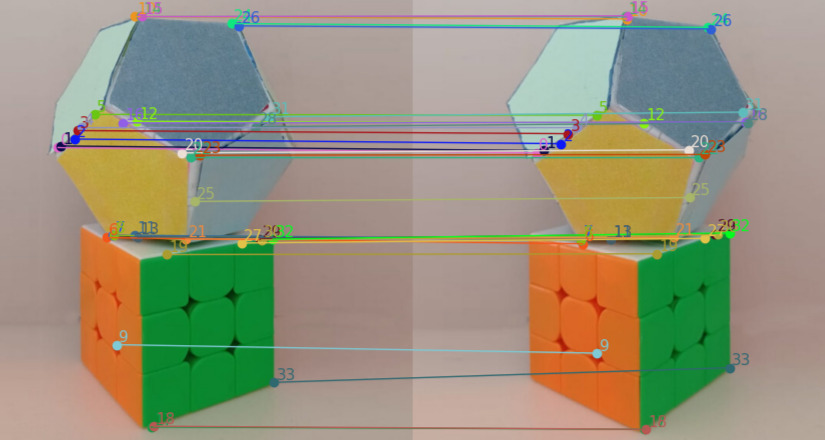
\includegraphics[width=\linewidth]{capture/app_complet_2.jpeg}\\
\hyperlink{brief-appendix}{
\beamerbutton{Seuil brief}
}
\hyperlink{sift-appendix}{
\beamerbutton{Comparaison avec Sift}
}
\end{center}

\end{frame}
